% !TEX root = ../Bachelorthesis.tex
%
%************************************************
% Einführung
%************************************************
\chapter{Einführung}
\label{sec:Einfuehrung}

Springer Nature ist ein weltweit führender Verlag für Forschungs-, Bildungs- und Fachliteratur mit einer breiten Palette an angesehenen und bekannten Marken und zudem der größte Verlag für Wissenschaftsbücher. Für Springer Nature ist es darum wichtig, auf ihren Web-Applikationen eine Suche anbieten zu können, die Suchintentionen erkennt und möglichst schnell zum gesuchten Content leitet. Die Suche wird vor allem als Hilfsmittel zur Navigation und Suche nach Literatur und Dienstleistungen genutzt. Durch die vielen von Springer Nature publizierten Zeitschriften und Querverweise in Artikeln, wird sie aber auch oft zur Suche nach Issues\footnote{Nummer der Zeitschriftenausgabe, in der sich der Artikel befindet.} und Artikeln verwendet sowie als Hilfestellung um Diagnosen zu Krankheitsbilder stellen zu können.
\\
\\
Springer Nature sammelt viele User-Tracking-Daten und dadurch viel Wissen über das Verhalten der User auf ihrer Suche, lässt dieses Wissen jedoch nicht in ihre Suche einfließen. In dieser Arbeit wird untersucht, wie mithilfe dieses Wissens, die Suche optimiert werden kann.

\section{Aufbau der Suche bei Springer Nature}
\label{sec:Einfuehrung:AufbauSucheBeiSpringerNature}

\subsubsection{White Label Applikation mit Solr-Suche}
\label{sec:Einfuehrung:AufbauSucheBeiSpringerNature:WhiteLabelApplikationSolr-Suche}

Damit die verschiedenen Verlage und Zeitschriften der Verlagsgruppe Springer Nature ihre Produkte und Dienstleistungen online anbieten können nutzt Springer Nature eine inhouse entwickelte White Label Applikation\footnote{\glqq weißes Etikett\grqq{} - eine nicht beschriftete Applikation, welche von anderen Firmen unter deren Namen verwendet werden kann}. Die White Label Applikation verwendet \textit{Apache Solr} als Suchplattform. Die Solr dient hierbei als eine der Schnittstellen zwischen dem Content-Pool von Springer und der Core-Applikation. Bei dem vom Content-Pool gelieferten Content, handelt es sich um vom Springer-Verlag publizierte Zeitschriften, Artikel, Bücher, Chapters und redaktionelle Inhalte.

\subsubsection{User-Tracking mit Webtrekk}
\label{sec:Einfuehrung:AufbauSucheBeiSpringerNature:Webtrekk}

Um das Verhalten der User auf ihren Web-Applikationen zu tracken verwendet Springer das Analysetool Webtrekk\footnote{https://www.webtrekk.com}. Die daraus resultierenden Reports bieten unter anderem die Möglichkeit, \textit{Suchquery-Logs} und \textit{Click-Trough-Rates}\footnote{Kennzahl um die Anzahl der Klicks auf Links im Verhältnis zu den gesamten Impressionen darzustellen} der User auszuwerten.

\pagebreak

\subsubsection{Architektur}
\label{sec:Einfuehrung:AufbauSucheBeiSpringerNature:rchitektur}

In Abb. \ref{fig:SucheSpringerNature} ist die Suche nochmals grafisch aufbereitet:

\begin{figure}[H]
\centering
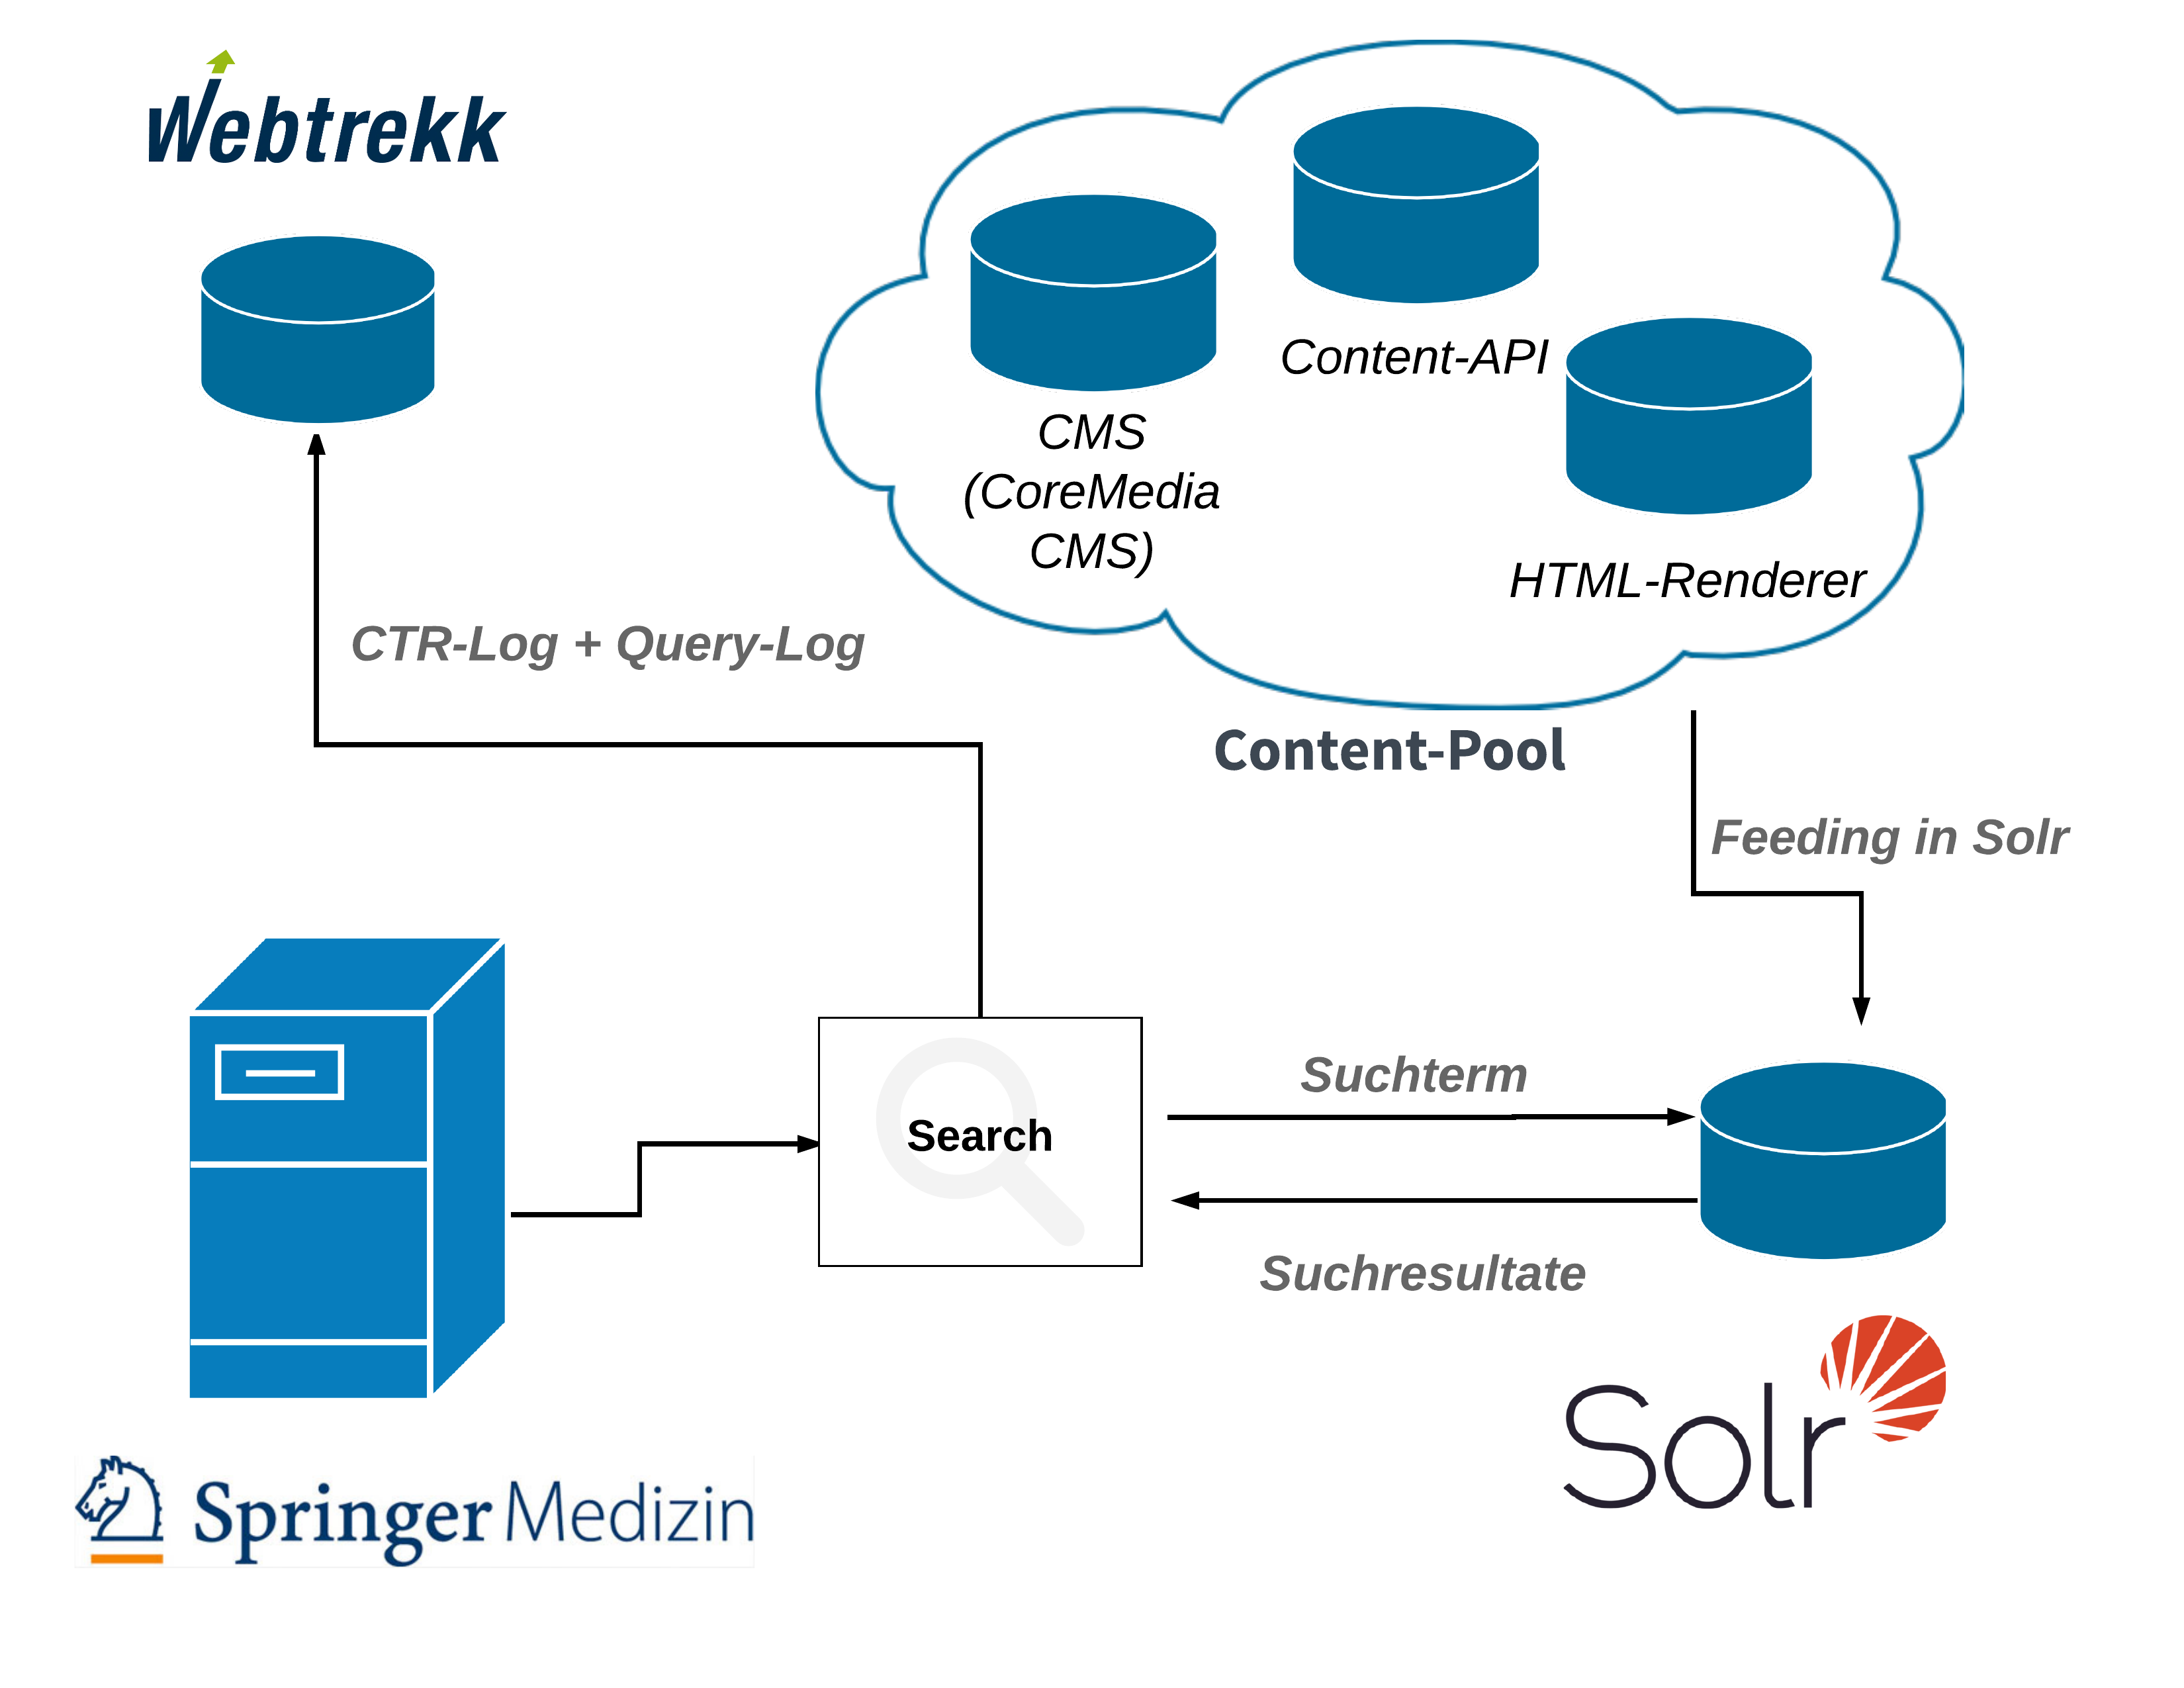
\includegraphics[width=0.5\linewidth]{gfx/AufbauSucheSpringerNature}
\caption[Aufbau der Suche bei Springer Nature]{Aufbau der Suche bei Springer Nature}
\label{fig:SucheSpringerNature}
\end{figure}

\section{Das große Problem}
\label{sec:Einfuehrung:Problemstellung}

\subsubsection{Der Springer Nature Stakeholder Springermedizin setzt auf Webtrekk}
\label{sec:Einfuehrung:Problemstellung:Springermedizin}

Zu den Stakeholder\footnote{bezeichnet Springer-interne Kunden, die ein Interesse am Ergebnis der White Label Applikation haben} der in \ref{sec:Einfuehrung:AufbauSucheBeiSpringerNature:WhiteLabelApplikationSolr-Suche} angesprochenen White Label Applikation gehört \textit{Springermedizin}\footnote{https://www.springermedizin.de/}. Springermedizin ist ein Fortbildungs- und Informationsportal für Ärzte. Mithilfe von Webanalysten und Webtrekk versucht Springermedizin das Marketing ihres Webauftrittes zu verbessern und ist sehr interessiert an neuen Ansätzen, um die gesammelten Tracking-Daten besser einzusetzen. In dieser Arbeit wird darum der Fokus auf die Suche von Springermedizin gesetzt. 

\subsubsection{Keine Userrelevanz in der Suche}
\label{sec:Einfuehrung:Problemstellung:Userrelevanz}

Die User von Springermedizin suchen oft mit einschlägig, fundierten Fachbegriffen nach den neuesten und relevantesten Zeitschriften, Bücher oder Publikationen. Die zeitlich aktuellsten Suchtreffer zu finden ist für Springermedizin kein Problem. Die für den User \textit{relevantesten} jedoch schon. 

\subsubsection{Der fast gläserne User}
\label{sec:Einfuehrung:Problemstellung:Glaeserne-User}

Springermedizin sammelt Tracking-Daten über jegliche Aktivitäten auf deren Applikationen und investiert Zeit und Geld in die Individualisierung der Analysedaten auf Webtrekk. Mittlerweile sind knapp 30 Custom-Parameter\footnote{Individuell erzeugte Parameter für Reports und Analysen} auf Webtrekk angelegt um genau die Daten zu tracken, die sie über das Verhalten der User auf ihrer Applikationen wissen wollen. Dadurch ensteht ein fast \glqq gläsernen User\grqq{}.

\section{Ziel der Arbeit}
\label{sec:Einfuehrung:ZielArbeit}

Durch die \textit{Click-Trough-Rates} der Suchergebnisse auf den Suchterm bezogen, können die für die Nutzer der Suche relevanten Dokumente im Suchresultat bevorzugt werden. Diese Click-Trough-Rates können direkt aus Webtrekk gelesen werden. 
\\
\\
Die Click-Trough-Rate als absoluten Wert für das \textit{Relevanzfeedback} zu nehmen, wäre jedoch falsch. Es muss davon ausgegangen werden, dass viele User der Qualität der Suchmaschine vertrauen und die Top-Suchresultate als die relevantesten Suchresultate betrachten. \cite{Joachims} Das Relevanzfeedback muss daher in Relation zu anderen Faktoren betrachtet werden um eine wirkliche Verbesserung der Suchergebnisqualität erzielen zu können. Ein interessanter Ansatz ist hierbei das \textit{position-based Model} (PBM). \cite{chuklin2015} Dieses geht davon aus, dass die Wahrscheinlichkeit, dass ein User ein Dokument wirklich genau analysiert bevor er es anklickt, davon abhängt wie \textit{schlecht} dieses Dokument im Suchresultat gerankt ist. Je \textit{schlechter} das Ranking des angeklickten Dokumentes ist, je \textit{höher} ist das Relevanzfeedback zu bewerten.
\\
\\
Wird nun mittels der oben erwähnten Click-Trough-Rate in Verbindung mit dem position-based Model, die Relevanz der angeklickten Dokumente berechnet und darauf basierend ein Sortier-Algorithmus für die von der Solr zurückgegebenen Suchresultate entwickelt, müsste davon ausgegangen werden, eine Verbessung der Suchergebnisqualität erzielen zu können. Ziel dieser Arbeit ist es darum die Verbesserung der Suchqualität mittels Einbezug dieser Relevanzberechnung zu messen. Wichtig ist hierbei auch kritisch zu hinterfragen wie gut und unter welchen Voraussetzungen diese Lösung produktiv eingesetzt werden kann.

\section{Methodik}
\label{sec:Einfuehrung:Methodik}

In der aufgestellten These werden \textit{Feedback-Strategien} für die Click-Trough-Rate Auswertung, wie in \cite{Joachims} beschrieben, nicht verwendet. Diese werden in der Thesis auch nicht beachtet. Ebenfalls wird von komplexen Lern-Algorithmen wie in \cite{IWUSBI} vorgestellt, abgesehen. Der neue Lösungsansatz greift auch nicht in die Suchquery der Solr-Abfrage ein sondern sortiert das Ergebnis der Solr-Suche neu.
\\
\\
Die Relevanzberechnung für die im Suchresultat ausgespielten Dokumente soll auf Basis des angesprochenen \textit{position-based Model} \cite{chuklin2015} umgesetzt werden. Die Wissensbasis für den Algorithmus bildet Webtrekk. Der Vorteil bei dieser Lösung ist, dass der Algorithmus nicht ständig neues Wissen lernen uns altes vergessen muss, sondern mit einem tagesaktuellen und über eine frei definierbare Periode terminiertes Wissens  arbeiten kann. Für die Bachelorthesis wird der Webtrekk-Account von \textit{Springermedizin.de} verwendet und pro Suchterm spezifische Analysen über einen vordefinierten Zeitraum (die letzten 30 Tage) durchgeführt. Über die Webtrekk-API können diese Analysen zur Laufzeit gelesen und verarbeitet werden. 
\\
\\
Wie bereits in Kapitel \ref{sec:Einfuehrung:ZielArbeit} angesprochen, wird der Nutzer der Suche durch die Top-Suchresultate beeinflusst. Um dem entgegenzuwirken wird mithilfe eines zusätzlichen Zufallsranking der Suchergebnisliste, die Relevanz der Dokumente beeinflusst, um von der Solr-Suche schlecht gerankte Ergebnisse auch in den Fokus des Nutzers zu rücken.
\\
\\
Das große Kernproblem der Überprüfung wird das Messen der Qualität der erzielten Suchergebnisse sein. Um die Verbesserung der Suchqualität durch die aufgestellte These messen zu können, werden Analysen benötigt, die aussagen, wie gut die Qualität der aktuellen Suche im Vergleich zum neuen Lösungsansatz ist, wie viel Verbesserung der Ansatz bringt und an welchen Schrauben noch etwas gedreht werden muss, damit die Suche wirklich gute Ergebnisse aus Sicht der User bringt. Dazu muss eine passende Testumgebung aufgebaut werden. Auf einem Evaluationssystem sollen fachlichen Experten die Relevanz der Suchergebnisse der beiden Suchmaschinen auf Basis gleicher Suchanfragen bewerten. Mithilfe des Bewertungsalgorithmus \textit{NDCG} kann dann anhand der Ergebnisse der Bewertungen, das Qualitätsmaß der beiden Suchen vergleichen und die Verbesserung der Suchqualität durch die neu implementierte Lösung festgestellt werden.

\section{Gliederung und Aufbau}
\label{sec:Einfuehrung:GliederungAufbau}

Wann lesen wir was und warum?